\chapter{Технологическая часть}

В данном разделе представлены требования к ПО, выбор средств реализации, реализации алгоритмов, описание интерфейса программы.

\section{Требования к ПО}
\begin{itemize}
	\item программа выполняет генерацию лесистой местности на основе таких параметров, как количество деревьев, координаты местности, густота кроны, ассиметрия дерева;
	\item программа позволяет отображать сгенерированную местность в различные этапы жизненного цикла деревьев;
	\item программа создает изображение на основе сгенерированной модели лесистой местности;
	\item программа может сохранять полученное изображение в файл формата \texttt{png};
	\item программа позволяет проводить модульное тестирование при запуске из командной строки;
	\item программа позволяет указывать количество потоков для работы при запуске из командной строки;
	\item программа выводит время, затраченное на построение изображения, при запуске из командной строки.
\end{itemize}

\subsection{Функциональная модель}
На рис. \ref{img:idef0_0}~--~\ref{img:idef0_1} представлена функциональная модель программы в нотации \texttt{IDEF0}.

\noindent
\begin{figure}[h!]
	\centering
    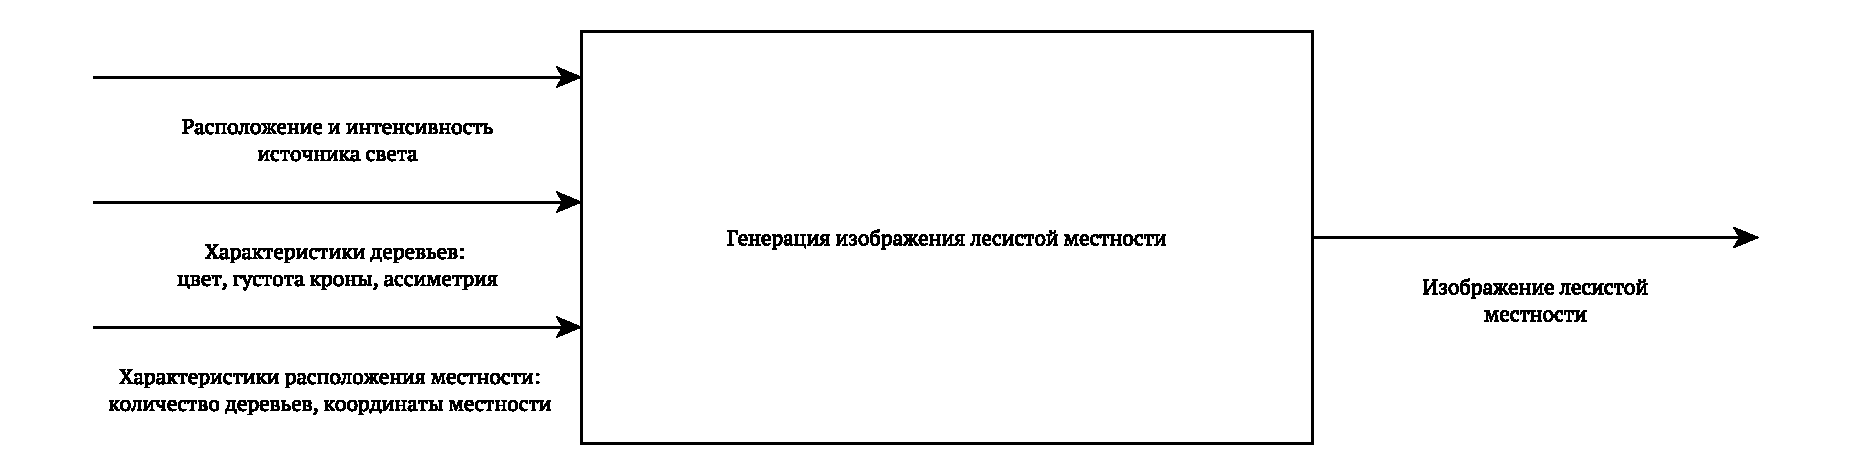
\includegraphics[width=1\linewidth]{idef0_0.pdf}
    \caption{Функциональная модель в нотации \texttt{IDEF0}}
    \label{img:idef0_0}
\end{figure}

\noindent
\begin{figure}[h!]
	\centering
    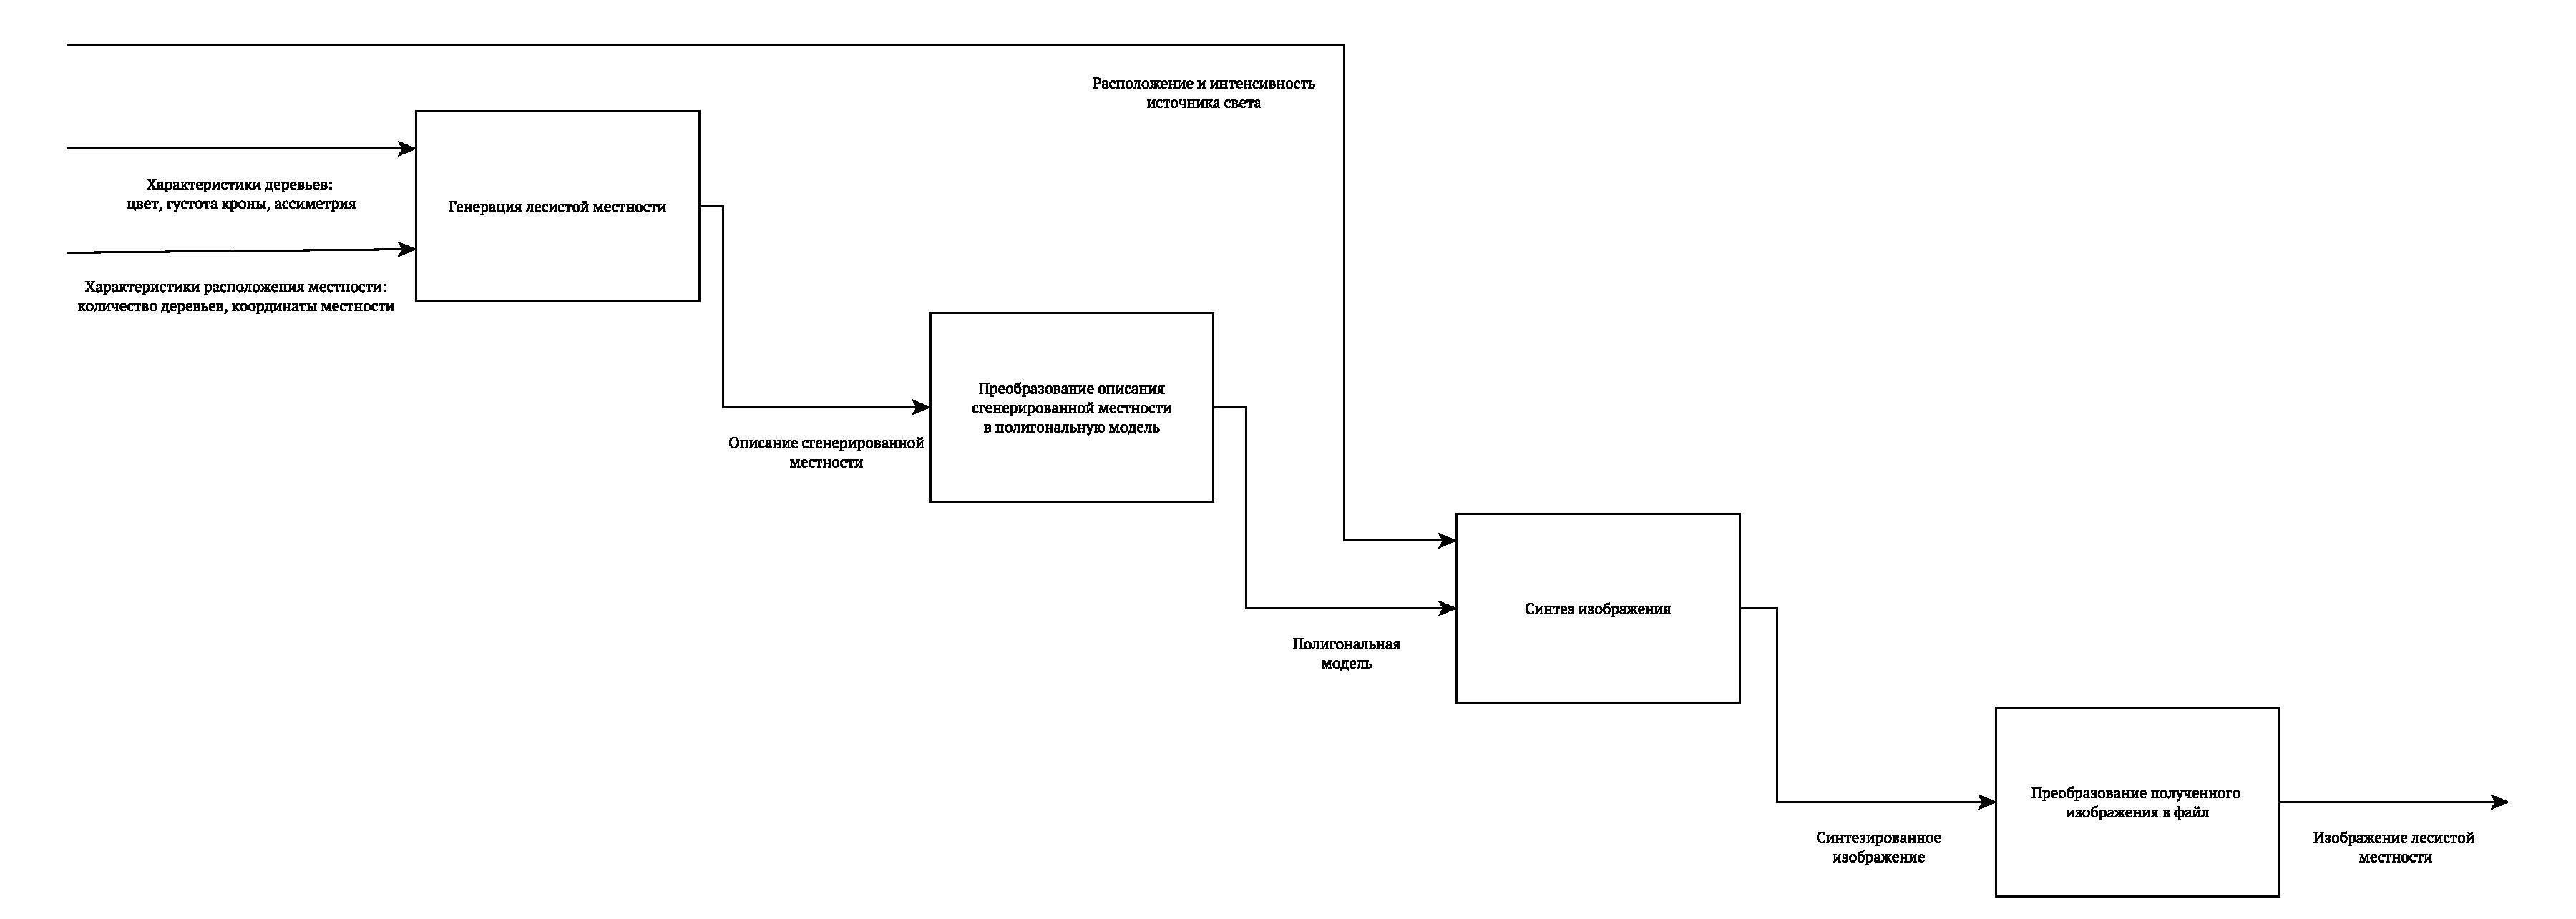
\includegraphics[width=1\linewidth]{idef0_1.pdf}
    \caption{Функциональная модель в нотации \texttt{IDEF0} (продолжение)}
    \label{img:idef0_1}
\end{figure}

\section{Средства реализации}

\subsection{Язык программирования}

В качестве языка программирования был выбран язык \texttt{C++}, так как он обладает достаточным инструментарием для работы с объектами, является компилируемым, имеет встроенные средства оценки времени работы программы.


\subsection{Набор библиотек}

В качестве набора библиотек был выбран \texttt{Qt}, так как он обладает достаточным инструменталом для работы с компьютерной графикой, а также имеет набор средств для создания кроссплатформенных графических приложений.

\subsection{Формат выходных файлов}
В качестве способа представления выходных данных был выбран формат \texttt{PNG}, так как он:

\begin{itemize}
	\item является кроссплатформенным, его можно просмотреть на любой популярной платформе без использования дополнительного программного обеспечения;
	\item обеспечивает качество изображения не худшее, чем в конкурирующих форматах, при приемлимом потреблении памяти файлом \cite{bib:14};
	\item поддерживается фреймворком \texttt{Qt}.
\end{itemize}

\section{Реализация алгоритма обратной трассировки лучей}

В листингах \ref{lst:1}~--~\ref{lst:4} представлена реализация алгоритма обратной трассировки лучей. 

\newpage
\begin{code}
\caption{Листинг функции, реализующей основной цикл прохода по пикселам}
\label{lst:1}
\begin{minted}{cpp}
std::shared_ptr<QImage> Scene::paint() {
    polygons = forest.toPolygons();
    
    auto image = std::make_shared<QImage>(width, height, 
    QImage::Format_RGB32);
    image->fill(Qt::black);
    
    QPainter painter(image.get());
    
    std::vector<std::vector<QColor>> colorBuffer(height,
    std::vector<QColor>(width, Qt::black));
    
    Ray ray = Ray(camera, QVector3D());
    
    for (int y = 0; y < height; y++) {
        for (int x = 0; x < width; x++) {
        ray.direction = (QVector3D(x, y, 0) - camera).normalized();
        colorBuffer[y][x] = traceRay(ray);
        }
    }
    
    for (int y = 0; y < height; y++) {
        for (int x = 0; x < width; x++) {
            painter.setPen(colorBuffer[y][x]);
            painter.drawPoint(x, y);
        }
    }
    
    return image;
}
\end{minted}
\end{code}

\newpage
\begin{code}
\caption{Листинг функции, реализующей трассировку одного луча}
\label{lst:2}
\begin{minted}{cpp}
QColor Scene::traceRay(const Ray &ray) {
    TraceRayData data;
    size_t index = 0;
    bool first = true;
    
    for (size_t i = 0; i < polygons.size(); i++) {
        auto res = polygons[i].traceRay(ray);
        if (!res.ok) {
            continue;
        }
        
        if (first || res.t < data.t) {
            index = i;
            data = res;
            first = false;
        }
    }
    
    if (first) {
        return background;
    }
    
    auto col = getColor(data.point, ray, lights, polygons[index]);
    if (!col.haveColor) {
        return Qt::black;
    }
    
    return col.color;
}
\end{minted}
\end{code}

\newpage
\begin{code}
\caption{Листинг функции, реализующей трассировку луча в рамках одного полигона}
\label{lst:3}
\begin{minted}{cpp}
TraceRayData Polygon::traceRay(const Ray &ray) {
    if (!shell.traceRay(ray)) {
        return TraceRayData();
    }

    QVector3D dir = ray.direction;
    QVector3D start = ray.camera;

    double k = a * dir.x() + b * dir.y() + c * dir.z();
    if (qFuzzyIsNull(k))
        return TraceRayData();

    double t = -(a * start.x() + b * start.y() + c * start.z() + d) / k;
    if (t < 0)
        return TraceRayData();

    QVector3D isc = start + dir * t;
    if (!inside(isc))
        return TraceRayData();

    return TraceRayData(isc, QVector3D(a, b, c).normalized(), t);
}
\end{minted}
\end{code}

\newpage
\begin{code}
\caption{Листинг функций, реализующих определение нахождения точки внутри полигона}
\label{lst:4}
\begin{minted}{cpp}
inline int sign(double a) {
    if (qFuzzyIsNull(a)) {
        return 0;
    }

    if (a > 0) {
        return 1;
    }

    return -1;
}

inline bool equalSign(double v1, double v2) {
    return sign(v1) * sign(v2) >= 0;
}

inline bool equalSigns(const QVector3D &v1, const QVector3D &v2) {
    return equalSign(v1.x(), v2.x()) && equalSign(v1.y(), v2.y()) 
    && equalSign(v1.z(), v2.z());
}

inline bool Polygon::inside(const QVector3D &p) {
    auto ap = p - pointA;
    auto bp = p - pointB;
    auto cp = p - pointC;

    auto m1 = QVector3D::crossProduct(ab, ap);
    auto m2 = QVector3D::crossProduct(bc, bp);
    auto m3 = QVector3D::crossProduct(ca, cp);

    return equalSigns(m1, m2) && equalSigns(m2, m3) && equalSigns(m3, m1);
}
\end{minted}
\end{code}

\section{Реализация алгоритма генерации лесистой местности}

В листингах \ref{lst:5}~--~\ref{lst:6} представлена реализация алгоритма генерации деревьев. В листингах \ref{lst:7}~--~\ref{lst:8} представлена реализация алгоритма перевода древовидной структуры сгенерированного дерева в полигональный формат. В листингах \ref{lst:9}~--~\ref{lst:10} представлена реализация алгоритма размещения деревьев на плоскости случайным образом.

\begin{code}
\caption{Листинг функции, реализующей рост дерева}
\label{lst:5}
\begin{minted}{cpp}
void Branch::grow(double feed) {
    radius = sqrt(area / M_PI);

    if (leaf) {
        double lenAddition = cbrt(feed);
        len += lenAddition;
        feed -= lenAddition * area;
        area += feed / len;
        if (canSplit()) {
            split();
        }
    } else {
        double childArea = childA->area + childB->area;
        double k = childArea / (childArea + area);
        area += k * feed / len;
        feed *= 1.0 - k;
        if (qFuzzyIsNull(k)) {
            return;
        }
        childA->grow(feed * ratio);
        childB->grow(feed * (1.0 - ratio));
    }
}
\end{minted}
\end{code}

\newpage
\begin{code}
\caption{Листинг функций, реализующих разделение ветви дерева}
\label{lst:6}
\begin{minted}{cpp}
double randSign() {
    return (rand() % 2) * 2 - 1;
}

QVector3D interpolate(QVector3D a, QVector3D b, double k) {
    return a * (1.0 - k) + b * k;
}

void Branch::split() {
    leaf = false;

    childA = new Branch(this, 0);
    childB = new Branch(this, 1);

    auto d = leafDensity(LOCAL_DEPTH);

    auto n = QVector3D::crossProduct(dir, d);
    n.normalize();

    auto m = -n;

    double flippedSpread = randSign() * spread;

    auto ns = n * flippedSpread;
    auto ms = m * flippedSpread;

    childA->dir = interpolate(ns, dir, ratio).normalized();
    childB->dir = interpolate(ms, dir, 1.0 - ratio).normalized();
}
\end{minted}
\end{code}

\newpage
\begin{code}
\caption{Листинг функции, производящей перевод дерева в полигональный формат}
\label{lst:7}
\begin{minted}{cpp}
std::vector<Polygon> Branch::toPolygons() {
    auto end = getEnd();
    auto x = dir + QVector3D(1.0, 1.0, 1.0);
    auto n = QVector3D::crossProduct(dir, x).normalized();
    double a = 180.0 / RING_POLYGONS;
    std::vector<Polygon> res;
    std::vector<QVector3D> positions;
    for (int i = 0; i < RING_POLYGONS; i++) {
        positions.push_back(start + radius * BRANCH_SCALE * n);
        n = rotateAboutVector(n, a, dir);
        positions.push_back(end + radius * BRANCH_SCALE * TAPER * n);
        n = rotateAboutVector(n, a, dir);
    }
    for (int i = 0; i < RING_POLYGONS; i++) {
        QVector3D a1 = positions[i * 2];
        QVector3D a2 = positions[(i * 2 + 2) % (2 * RING_POLYGONS)];
        QVector3D a3 = positions[i * 2 + 1];
        QVector3D b1 = positions[(i * 2 + 2) % (2 * RING_POLYGONS)];
        QVector3D b2 = positions[(i * 2 + 3) % (2 * RING_POLYGONS)];
        QVector3D b3 = positions[i * 2 + 1];
        res.push_back(Polygon(a1, a2, a3, color, Qt::white));
        res.push_back(Polygon(b1, b2, b3, color, Qt::white));
    }
    if (leaf && depth > 2) {
        QVector3D a1 = end + dir * 10;
        QVector3D a2 = end + n * 10;
        QVector3D a3 = end - n * 10;
        res.push_back(Polygon(a1, a2, a3, leafColor, Qt::white));
    }
\end{minted}
\end{code}

\newpage
\begin{code}
\caption{Листинг функции, производящей перевод дерева в полигональный формат (продолжение листинга \ref{lst:7})}
\label{lst:8}
\begin{minted}{cpp}
    if (leaf) {
        return res;
    }
    auto polygonsA = childA->toPolygons();
    auto polygonsB = childB->toPolygons();
    res.insert(res.end(), polygonsA.begin(), polygonsA.end());
    res.insert(res.end(), polygonsB.begin(), polygonsB.end());
    return res;
}
\end{minted}
\end{code}

\begin{code}
\caption{Листинг функции, генерирующей случайное размещение деревьев}
\label{lst:9}
\begin{minted}{cpp}
Forest::Forest(int n, int seed, QVector2D bl, QVector2D tr, double y,
 QColor tc, QColor lc, QColor pc, double r, double s, double ss):
    bottomLeft(bl),
    topRight(tr),
    treeColor(tc),
    leafColor(lc),
    planeColor(pc),
    ratio(r),
    spread(s),
    splitSize(ss),
    y(y)
{
    srand(seed);
    if (n > 0) {
        int trX = tr.x() - GAP;
        int trY = tr.y() - GAP;
        int blX = bl.x() + GAP;
        int blY = bl.y() + GAP;
\end{minted}
\end{code}

\newpage
\begin{code}
\caption{Листинг функции, генерирующей случайное размещение деревьев (продолжение листинга \ref{lst:9})}
\label{lst:10}
\begin{minted}{cpp}
        double shape = abs((trX - blX) * (trY - blY));
        double sOne = K * shape / n;
        double rad = sqrt(sOne / M_PI);
        std::vector<QVector2D> ps(shape);
        int i = 0;
        for (int y = blY; y < trY; y++) {
            for (int x = blX; x < trX; x++) {
                ps[i] = QVector2D(x, y);
                i++;
            }
        }
        std::default_random_engine e(seed);
        std::shuffle(ps.begin(), ps.end(), e);
        int size = ps.size();
        for (int i = 0; i < n && size > 0; i++) {
            auto pos = ps[rand() % size];
            trees.push_back(new Branch(QVector3D(pos.x(), y, pos.y()),
             ratio, spread, splitSize, treeColor, leafColor));
            for (int j = 0; j < size; j++) {
                if (ps[j].distanceToPoint(pos) <= rad) {
                    std::swap(ps[j], ps[size - 1]);
                    size--;
                }
            }
        }
    }
    bottomRight = QVector2D(topRight.x(), bottomLeft.y());
    topLeft = QVector2D(bottomLeft.x(), topRight.y());
}
\end{minted}
\end{code}

\section{Описание интерфейса программы}
Программа запускается или из среды разработки \texttt{Qt Creator}, или с помощью командной строки. На рис. \ref{img:interface} представлен внешний вид основного окна программы.

\noindent
\begin{figure}[h!]
	\centering
    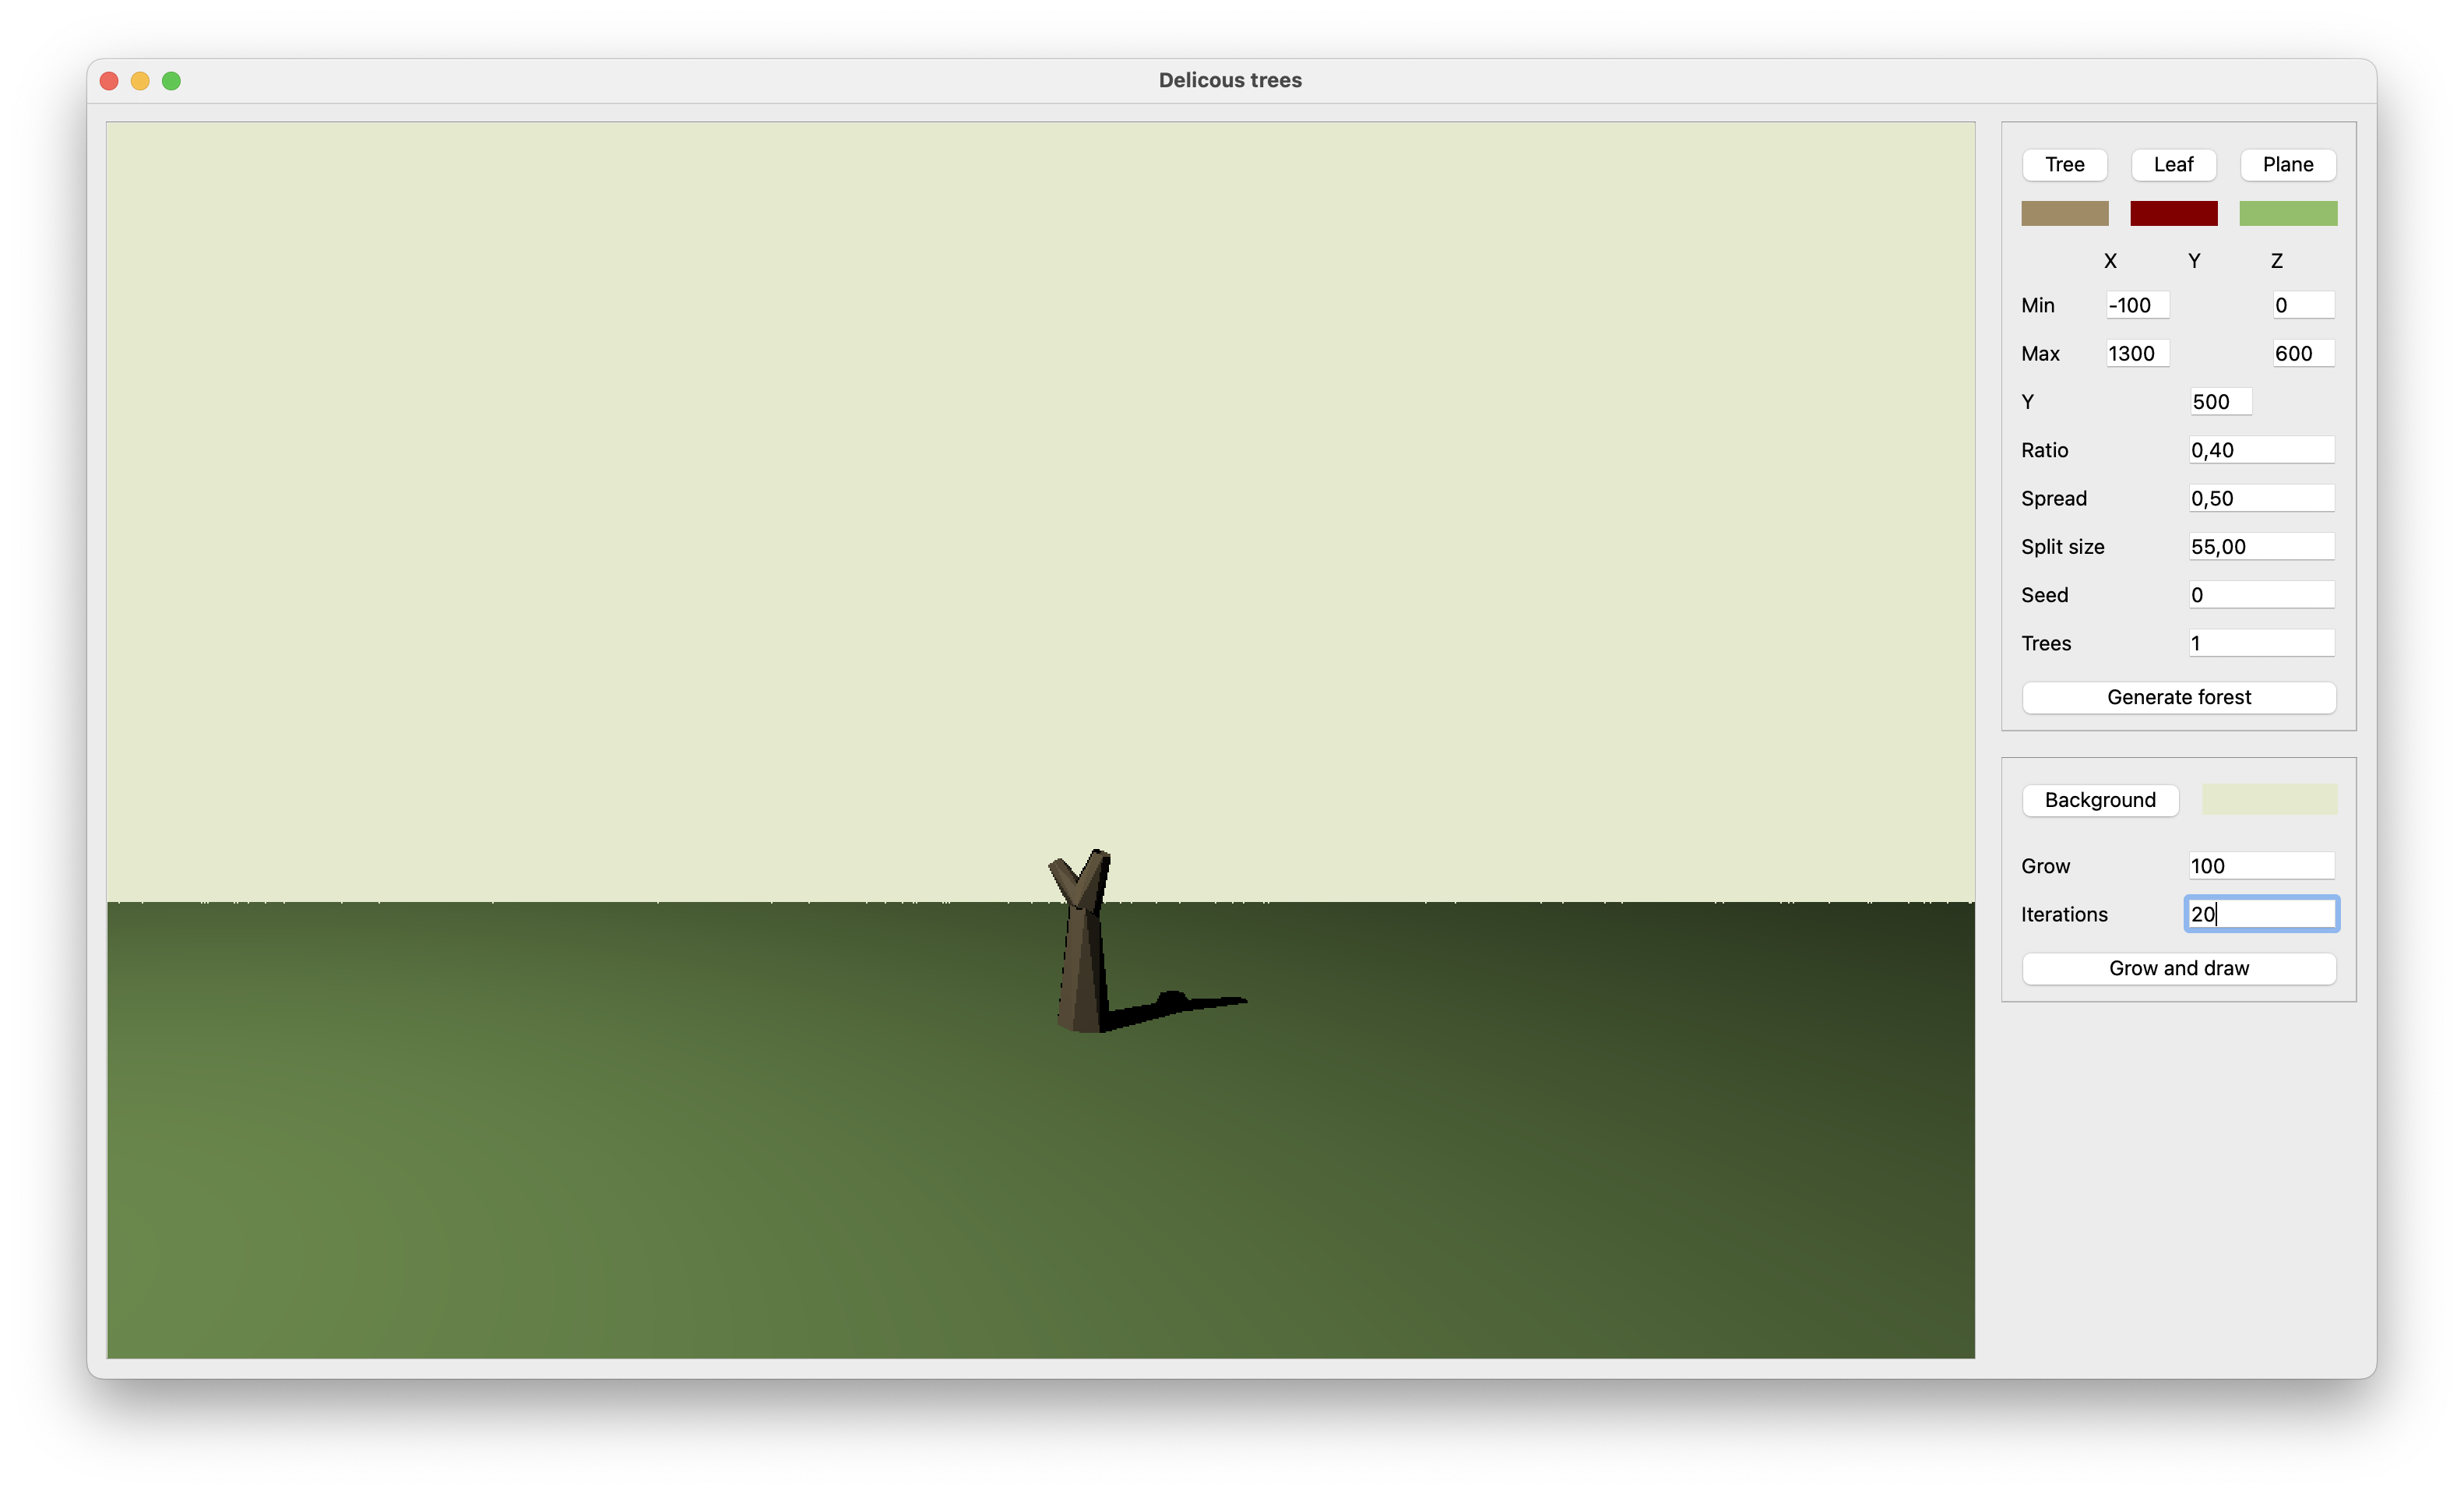
\includegraphics[width=1\linewidth]{interface.png}
    \caption{Внешний вид основного окна программы}
    \label{img:interface}
\end{figure}

\begin{itemize}
\item \texttt{Tree}~---~кнопка для изменения цвета деревьев;
\item \texttt{Leaf}~---~кнопка для изменения цвета листьев;
\item \texttt{Plane}~---~кнопка для изменения цвета площадки под деревьями;
\item \texttt{Min}~---~минимальные координаты плоскости по $x$ и $z$;
\item \texttt{Max}~---~максимальные координаты плоскости по $x$ и $z$;
\item \texttt{Y}~---~координата $y$ плоскости;
\item \texttt{Ratio}~---~соотношение объема питания одной ветки к другой;
\item \texttt{Spread}~---~густота кроны;
\item \texttt{Split size}~---~длина ствола, после которого он начнет разделяться;
\item \texttt{Seed}~---~зерно случайной генерации;
\item \texttt{Trees}~---~количество деревьев;
\item \texttt{Generate forest}~---~кнопка для генерации нового леса;
\item \texttt{Background}~---~кнопка для изменения цвета фона;
\item \texttt{Grow}~---~количество питания, поставляемого деревьям;
\item \texttt{Iterations}~---~количество итераций, в течение которых деревьям будет доставлено указанное количество питания;
\item \texttt{Grow and draw}~---~кнопка для доставки питания к деревьям и отрисовки сцены.
\end{itemize}

\section{Описание управления из командной строки}

Программа поддерживает аргументы командной строки. Ниже представлено их описание.

\begin{itemize}
	\item \texttt{-i}~---~количество итераций, в течение которых деревьям будет доставлено питание;
	\item \texttt{-o}~---~название выходного файла;
	\item \texttt{-u}~---~если указан, то проводится модульное тестирование;
	\item \texttt{-b}~---~если указан, то программа осуществляет замер времени;
	\item \texttt{-t}~---~количество потоков, используемых при синтезе изображения.
\end{itemize}

\section{Тестирование}

Тестирование программы проводилось с использованием модульных тестов. 
Для модульного тестирования использовалась библиотека \texttt{Qt Test}.
Для каждого тестируемого класса \texttt{Class} создается класс \texttt{TestClass}, наследуемый от \texttt{QObject}. Конкретные тесты помещаются в приватные слоты этого класса.

Соответственно, для добавления новых тестов, необходимо создать класс тестирования (если такового нет), и добавить тесты в его приватные слоты.

В листингах \ref{lst:11}~--~\ref{lst:12} приведены примеры тестового класса и тестовой функции.

\begin{code}
\caption{Класс тестирования полигона}
\label{lst:11}
\begin{minted}{cpp}
class TestPolygon : public QObject
{
    Q_OBJECT
public:
    explicit TestPolygon(QObject *parent = nullptr);

private slots:
    void test_traceRay_usual();

signals:

};
\end{minted}
\end{code}

\begin{code}
\caption{Функция тестирования}
\label{lst:12}
\begin{minted}{cpp}
void TestPolygon::test_traceRay_usual() {
    auto p = Polygon(QVector3D(0, 0, 0), 
    QVector3D(100, 0, 0), QVector3D(0, 100, 0), 
    Qt::black, Qt::black);

    Ray ray = Ray(QVector3D(0, 0, 100), QVector3D(0, 0, -1));
    auto resp = p.traceRay(ray);

    QCOMPARE(resp.ok, true);
    QCOMPARE(qFuzzyCompare(resp.t, 100), true);
}
\end{minted}
\end{code}

\section{Примеры работы программы}
На рисунках \ref{img:example1}~--~\ref{img:example4} показаны примеры работы программы для различных входных параметров.

\newpage 

\noindent
\begin{figure}[h!]
	\centering
    \includegraphics[width=0.9\linewidth]{example1.png}
    \caption{Обычное дерево}
    \label{img:example1}
\end{figure}

\noindent
\begin{figure}[h!]
	\centering
    \includegraphics[width=0.9\linewidth]{example2.png}
    \caption{Дерево в японском стиле}
    \label{img:example2}
\end{figure}

\newpage 

\noindent
\begin{figure}[h!]
	\centering
    \includegraphics[width=0.9\linewidth]{example3.png}
    \caption{Дерево в северном стиле}
    \label{img:example3}
\end{figure}

\noindent
\begin{figure}[h!]
	\centering
    \includegraphics[width=0.9\linewidth]{example4.png}
    \caption{Небольшой лес}
    \label{img:example4}
\end{figure}

\newpage 

\section{Выводы по технологической части}
В данном разделе была рассмотрена реализация алгоритмов обратной трассировки лучей и генерации лесистой местности. Был разобран интерфейс программы, флаги командной строки, модульное тестирование. Кроме того, были показаны примеры работы программы на различных входных данных.

\newpage